\chapter{Concentration Metrics for the Zipfian Datasets}\label{ch:apdd}

\markboth{Appendix D}{}

Chapter~\ref{ch:technical} introduces the Zipfian family of training distributions parametrised by the concentration $\alpha$, and characterises how concentration grows with $\alpha$ through the KL divergence with respect to the uniform baseline. This appendix reports four additional aggregate measures of concentration computed on the same distributions: Shannon entropy, the Gini coefficient, Simpson diversity, and the imbalance ratio. All four are computed on the pair frequency distribution of a representative seed (seed 42), at every $\alpha$ in the range from 0.00 to 3.00. Because the distribution is Zipfian by construction, these measures are not independent findings but a verification: their agreement across $\alpha$ confirms that the intended concentration effect manifests consistently under several standard measures of inequality.

\section{Shannon Entropy}
\label{sec:appendix-shannon-entropy}

Shannon entropy measures the total uncertainty of a distribution. Applied to the pair frequency distribution, it is high when the training mass is spread over many pairs at comparable frequencies, and low when a few pairs absorb most of the exposures.

\begin{figure}[htbp]
    \centering
    \IfFileExists{images/shannon_vs_alpha.png}{%
        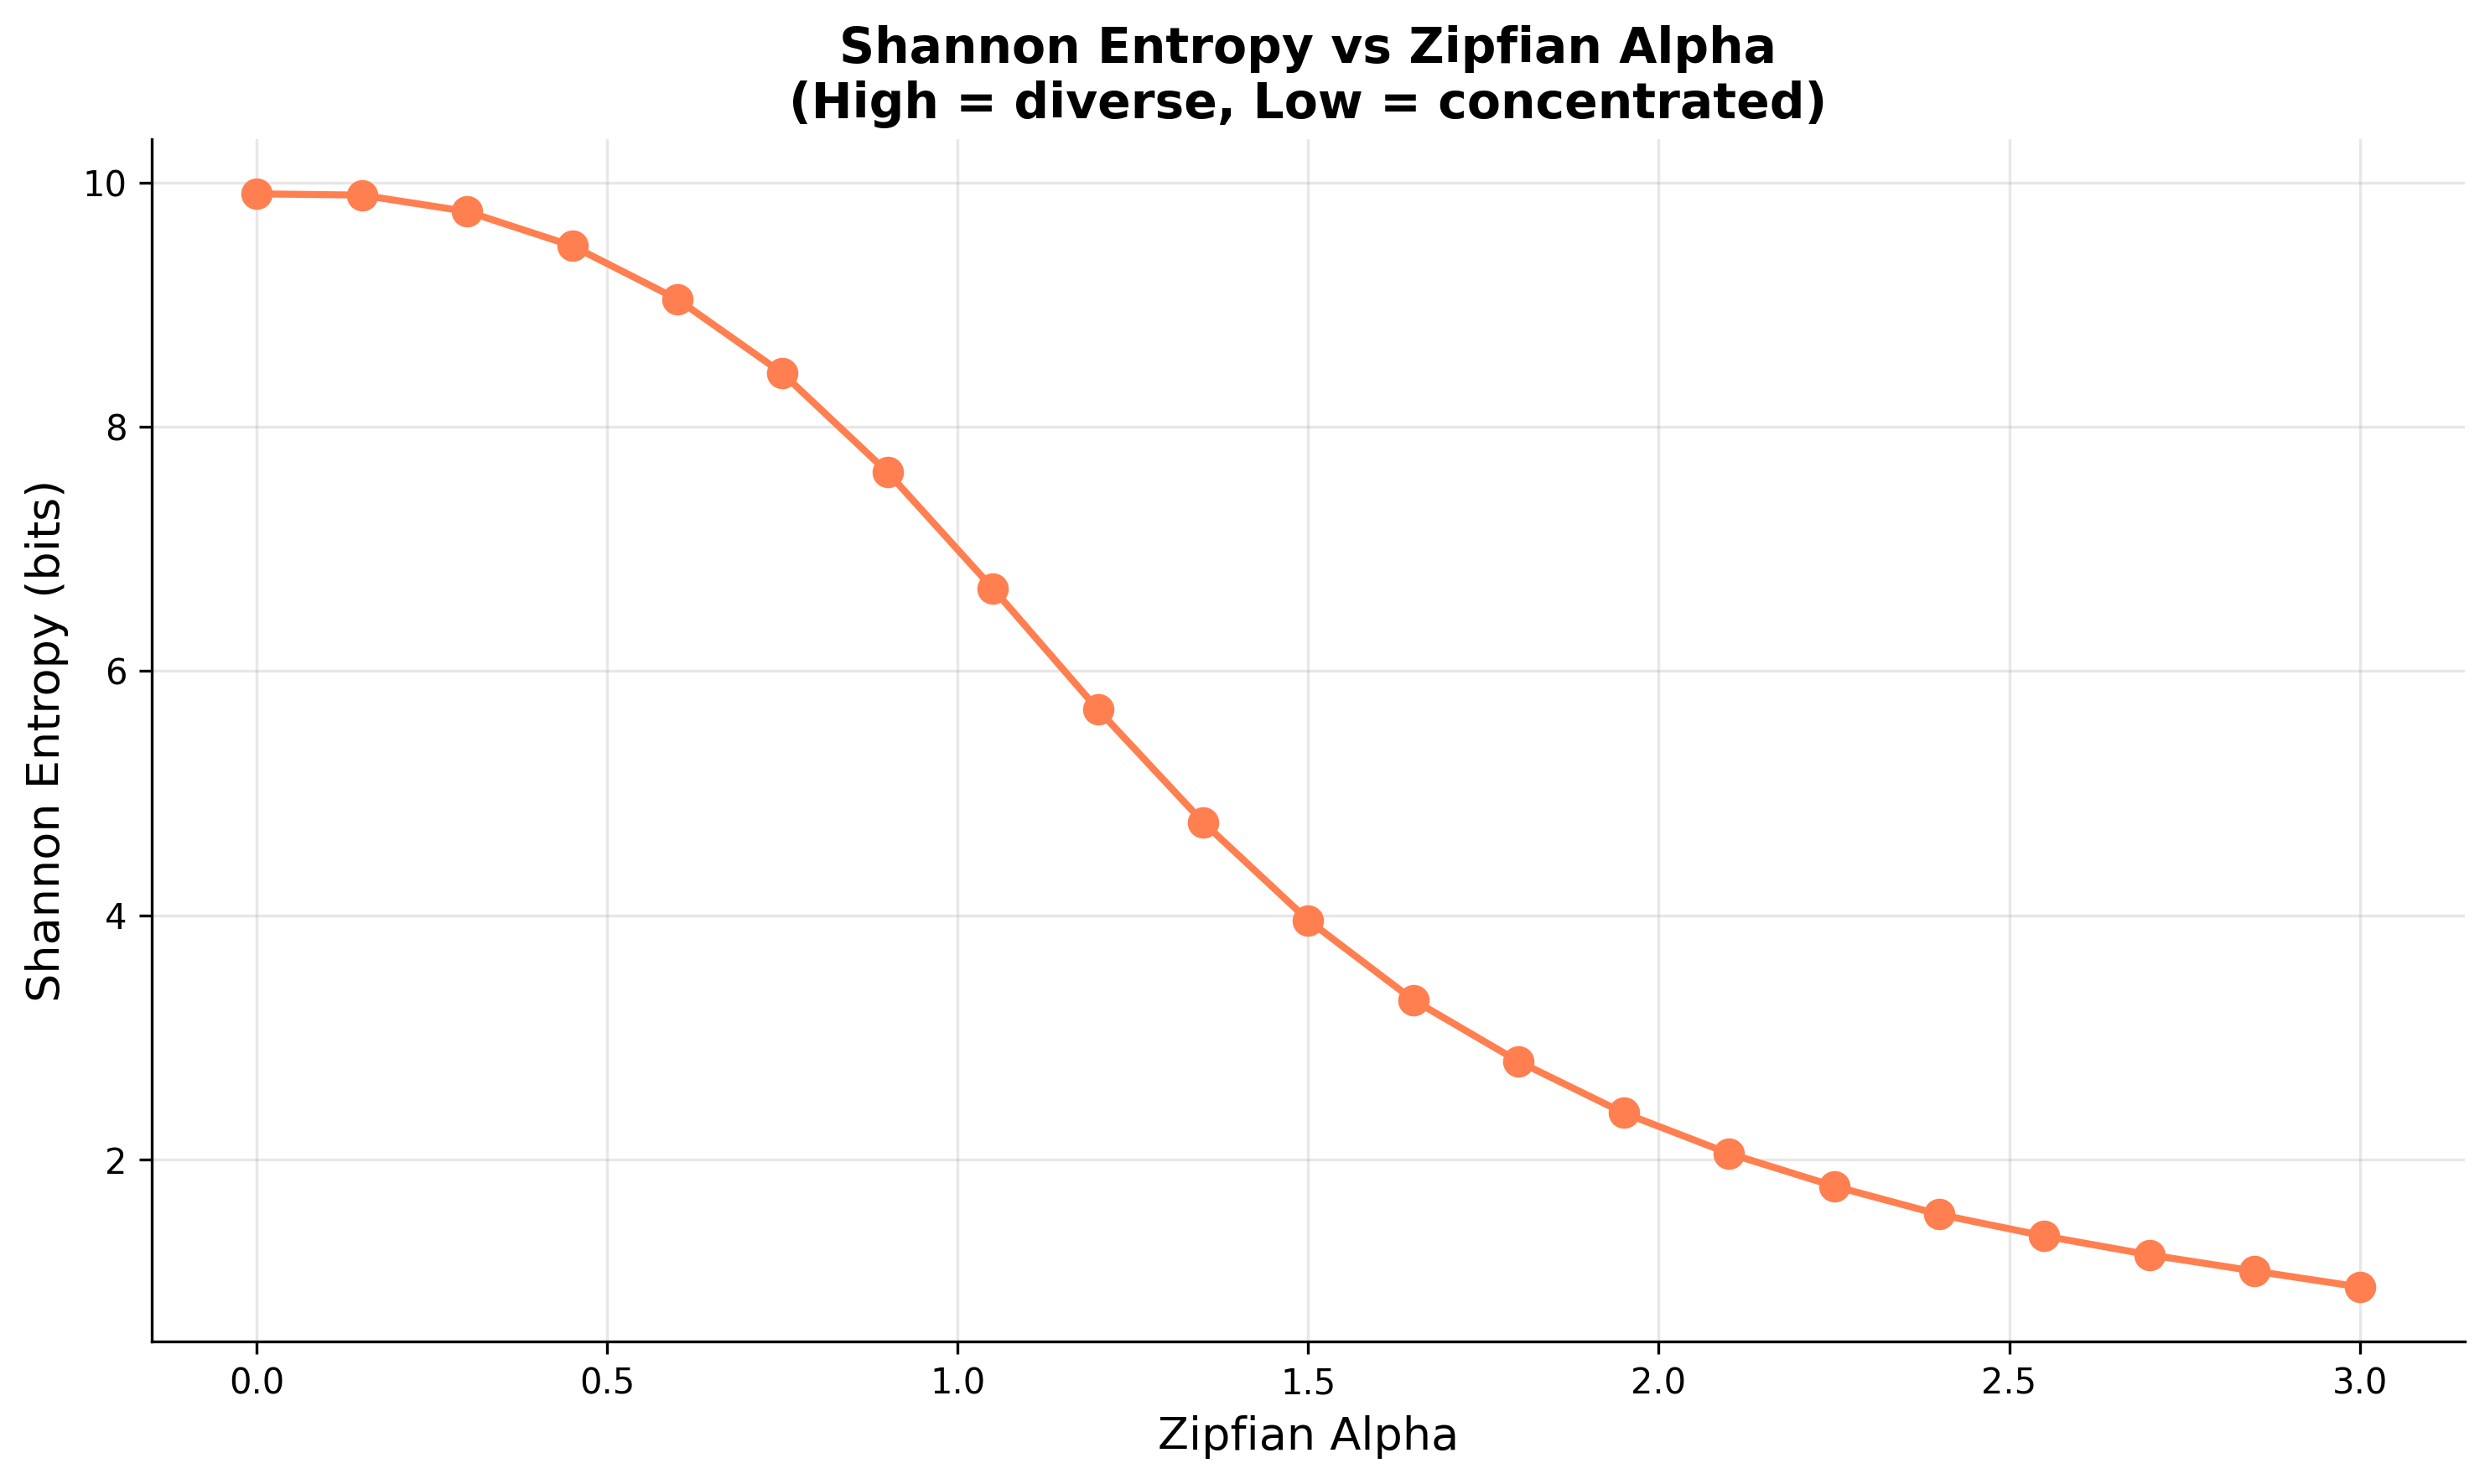
\includegraphics[width=0.95\textwidth]{images/shannon_vs_alpha.png}%
    }{%
        \fcolorbox{red}{white}{\parbox[c][0.14\textheight][c]{0.9\textwidth}{\centering\textcolor{red}{Placeholder figure\\\texttt{\detokenize{images/shannon_vs_alpha.png}}}}}%
    }
    \caption{Shannon entropy of the pair frequency distribution as a function of $\alpha$, computed on the training set of seed 42. The y-axis reports entropy in nats.}
    \label{fig:appendix-shannon-vs-alpha}
\end{figure}

The entropy decreases steadily with $\alpha$: as concentration grows, the training distribution weights the 961 possible pairs increasingly unequally, and the uncertainty about which pair a randomly drawn training example refers to falls accordingly.

\section{Gini Coefficient}
\label{sec:appendix-gini-coefficient}

The Gini coefficient is a classical measure of statistical inequality, ranging from 0 (perfect equality, every pair has the same frequency) to 1 (maximum inequality, one pair accounts for all the probability mass). Applied to the pair frequency distribution, a low Gini means the Zipfian dataset weights the 961 possible pairs almost equally; a high Gini means a small subset of pairs absorbs most of the training exposures.

\begin{figure}[htbp]
    \centering
    \IfFileExists{images/appendix_gini_vs_alpha.png}{%
        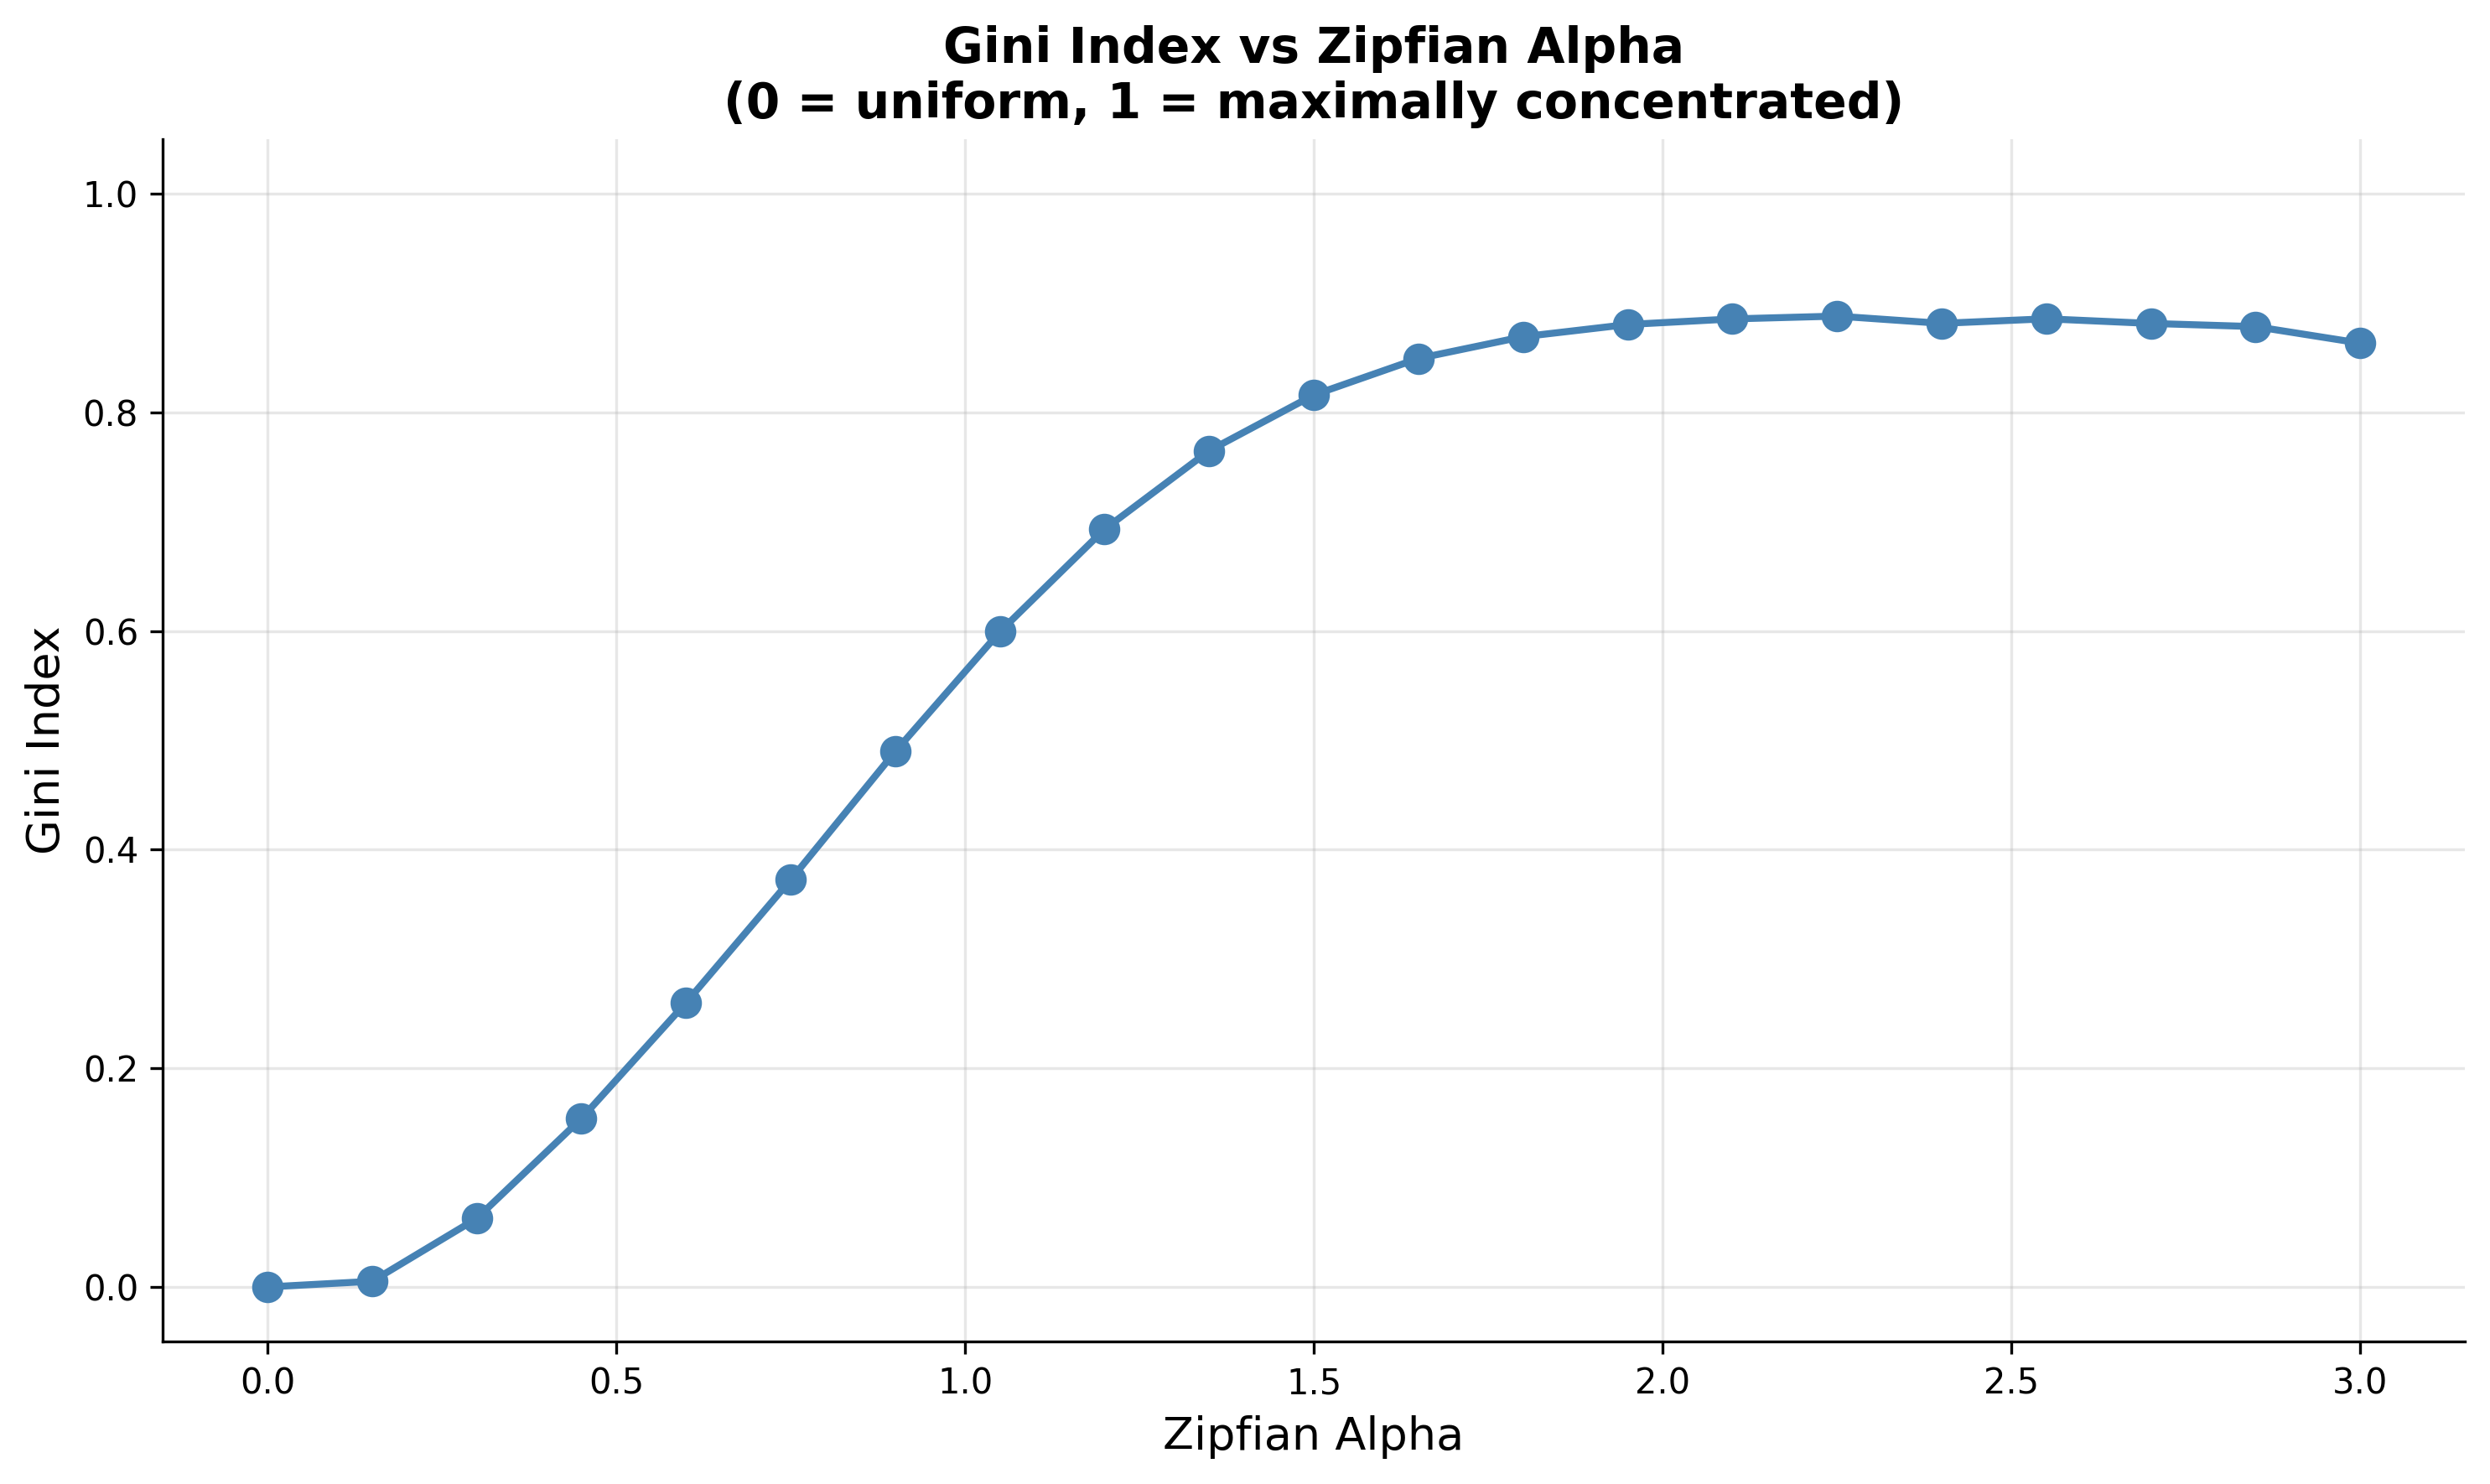
\includegraphics[width=0.95\textwidth]{images/appendix_gini_vs_alpha.png}%
    }{%
        \fcolorbox{red}{white}{\parbox[c][0.14\textheight][c]{0.9\textwidth}{\centering\textcolor{red}{Placeholder figure\\\texttt{\detokenize{images/appendix_gini_vs_alpha.png}}}}}%
    }
    \caption{Gini coefficient of the pair frequency distribution as a function of $\alpha$, computed on the training set of seed 42.}
    \label{fig:appendix-gini-vs-alpha}
\end{figure}

The Gini coefficient increases monotonically with $\alpha$, reflecting the same pattern captured by Shannon entropy. At low concentration, the Gini is close to zero, indicating a fairly even weighting of pairs across the training set. At high concentration, the Gini rises towards one, indicating that most of the training mass is concentrated on a small subset of pairs.

\section{Simpson Diversity Index}
\label{sec:appendix-simpson-diversity}

The Simpson diversity index measures the probability that two pair occurrences drawn at random from the training distribution correspond to different pairs. It ranges from 0 (all probability mass is assigned to one pair, no diversity) towards 1 (the mass is spread over many pairs, high diversity). Unlike the Gini coefficient, which measures aggregate inequality, Simpson diversity measures how many pairs are effectively distinct at the level of sampling.

\begin{figure}[htbp]
    \centering
    \IfFileExists{images/appendix_simpson_vs_alpha.png}{%
        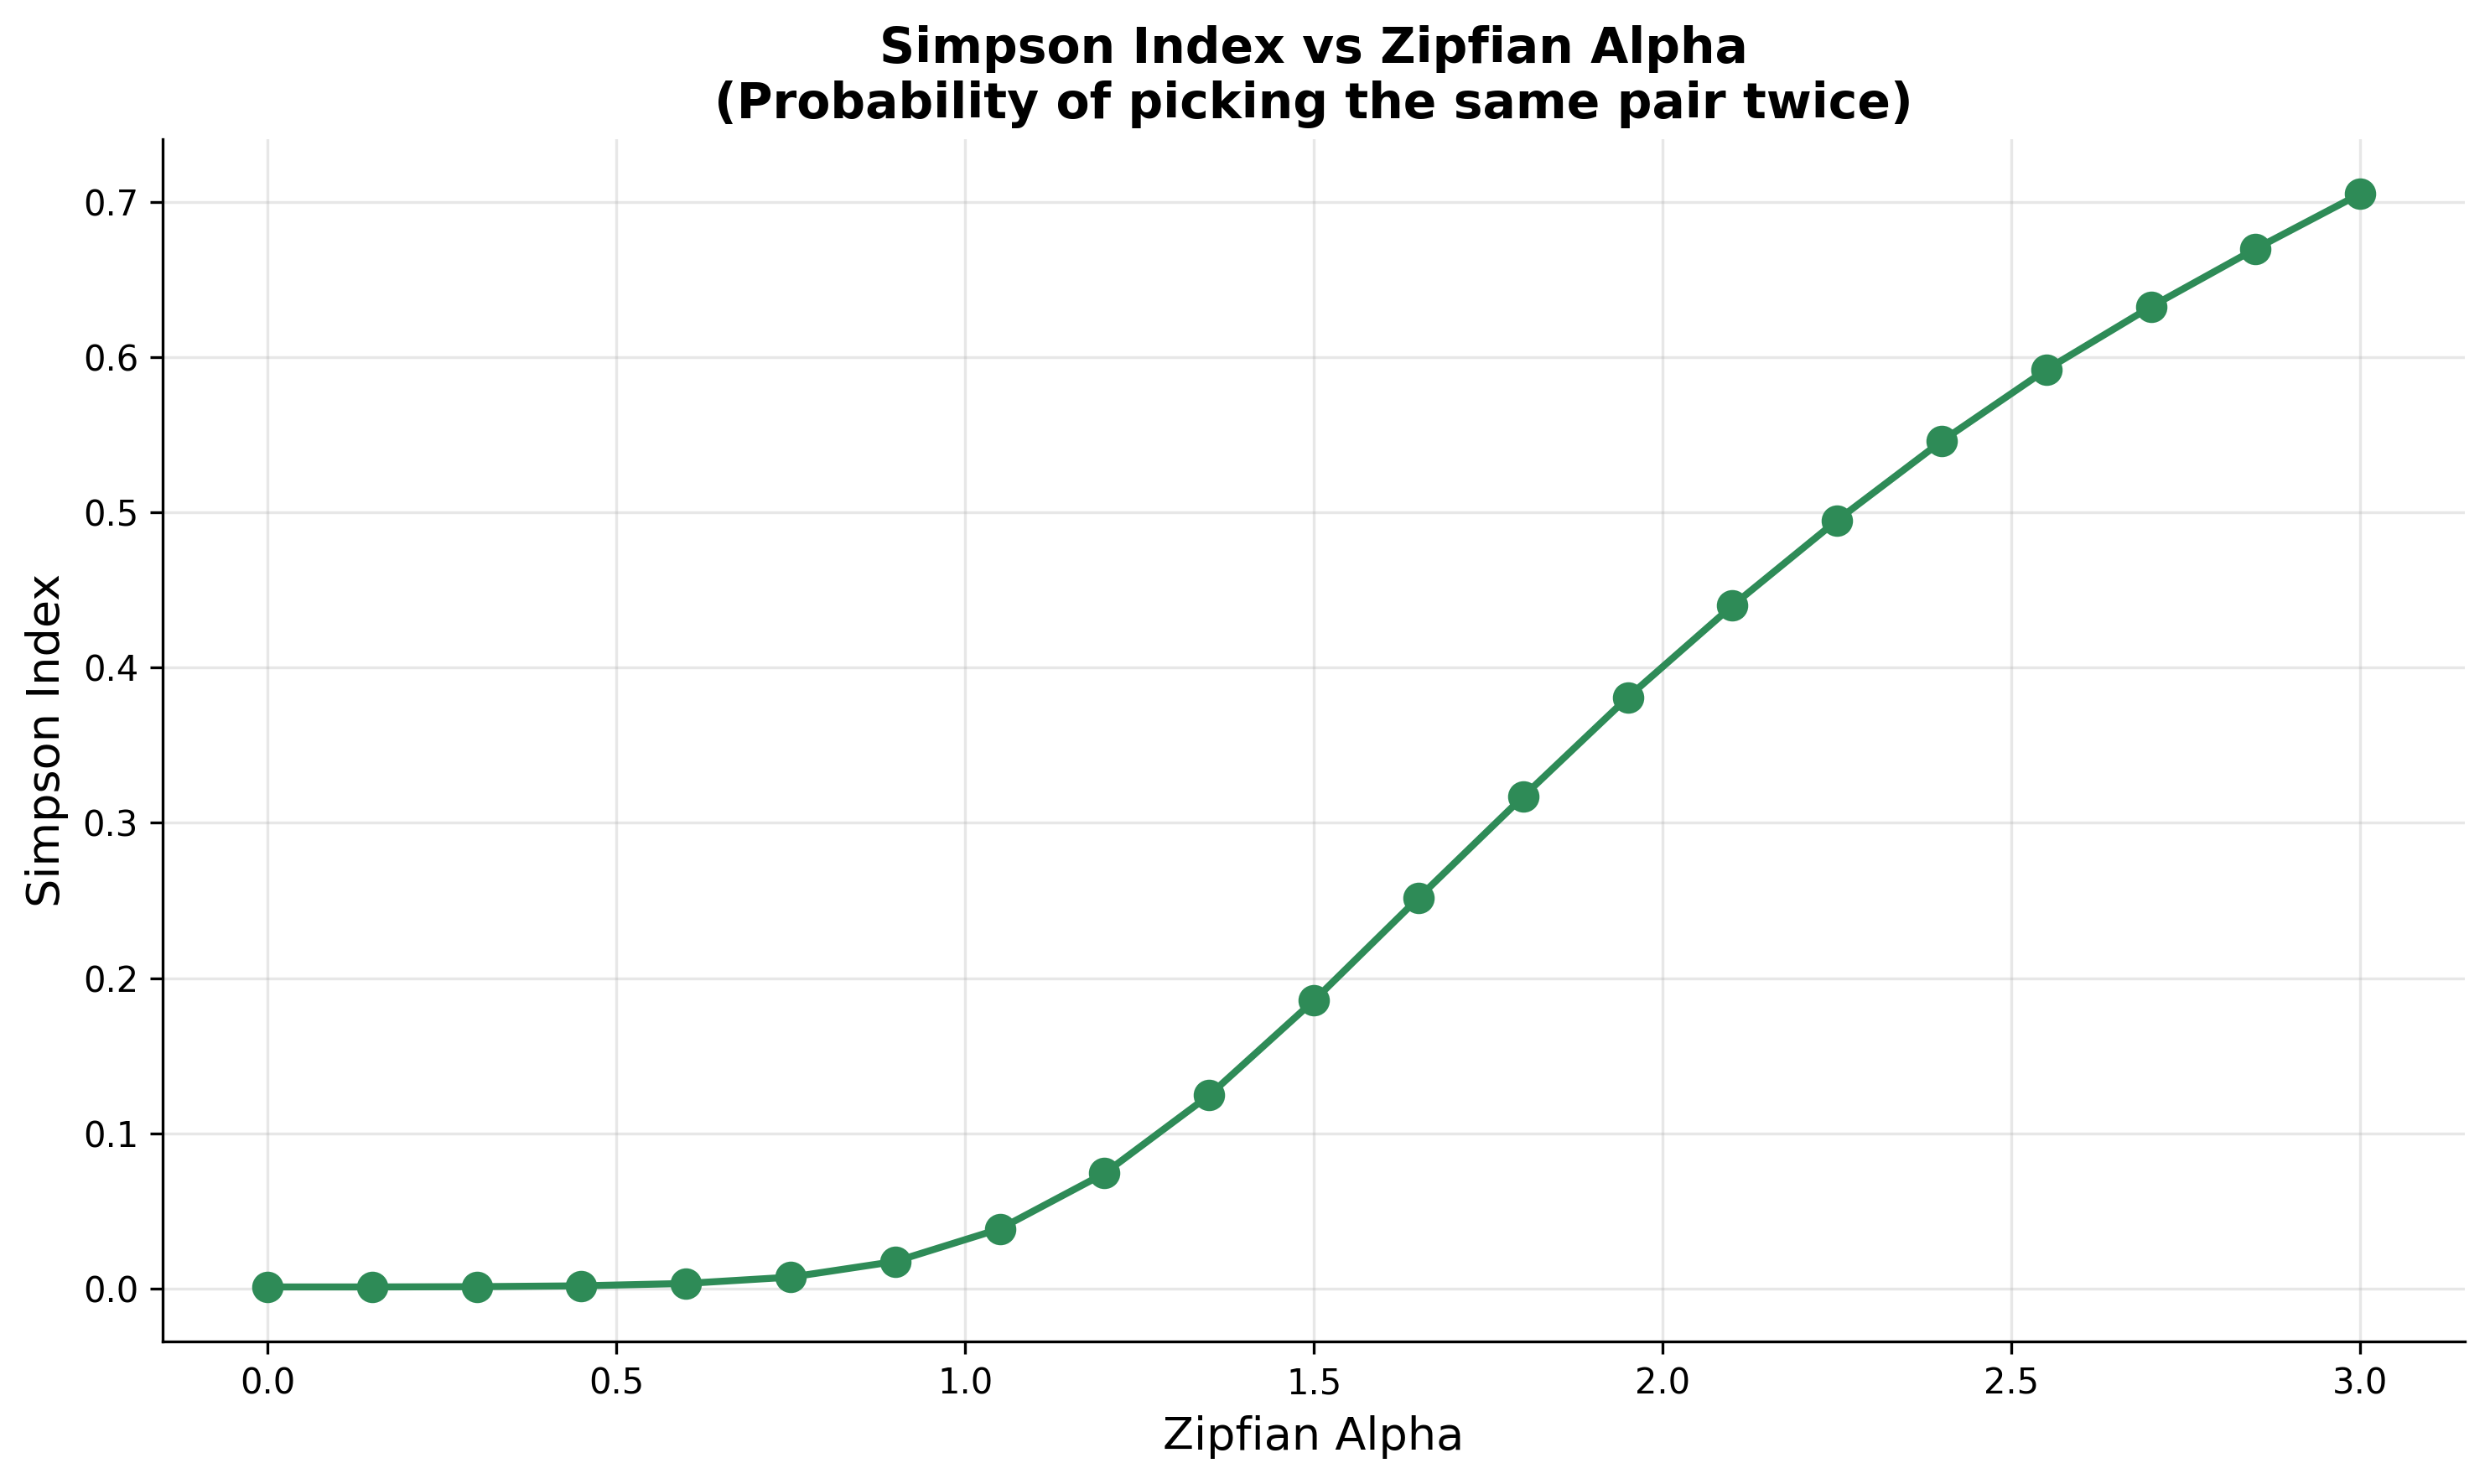
\includegraphics[width=0.95\textwidth]{images/appendix_simpson_vs_alpha.png}%
    }{%
        \fcolorbox{red}{white}{\parbox[c][0.14\textheight][c]{0.9\textwidth}{\centering\textcolor{red}{Placeholder figure\\\texttt{\detokenize{images/appendix_simpson_vs_alpha.png}}}}}%
    }
    \caption{Simpson diversity of the pair frequency distribution as a function of $\alpha$, computed on the training set of seed 42.}
    \label{fig:appendix-simpson-vs-alpha}
\end{figure}

Simpson diversity decreases monotonically with $\alpha$. In practical terms, at $\alpha = 0.00$ two randomly drawn training examples almost always refer to different pairs, while at $\alpha = 3.00$ the effective diversity has fallen to roughly 30\% of its uniform value: a handful of top-ranked pairs accounts for a large share of the draws.

\section{Imbalance Ratio}
\label{sec:appendix-imbalance-ratio}

The imbalance ratio is the ratio between the frequency of the most common pair and that of the least common pair. It is unbounded above and takes value 1 when every pair is equally frequent. Unlike Gini and Simpson, which are aggregate measures, the imbalance ratio focuses specifically on the tail: how much more often the dominant pairs appear compared to the rarest ones.

\begin{figure}[htbp]
    \centering
    \IfFileExists{images/appendix_imbalance_ratio_vs_alpha.png}{%
        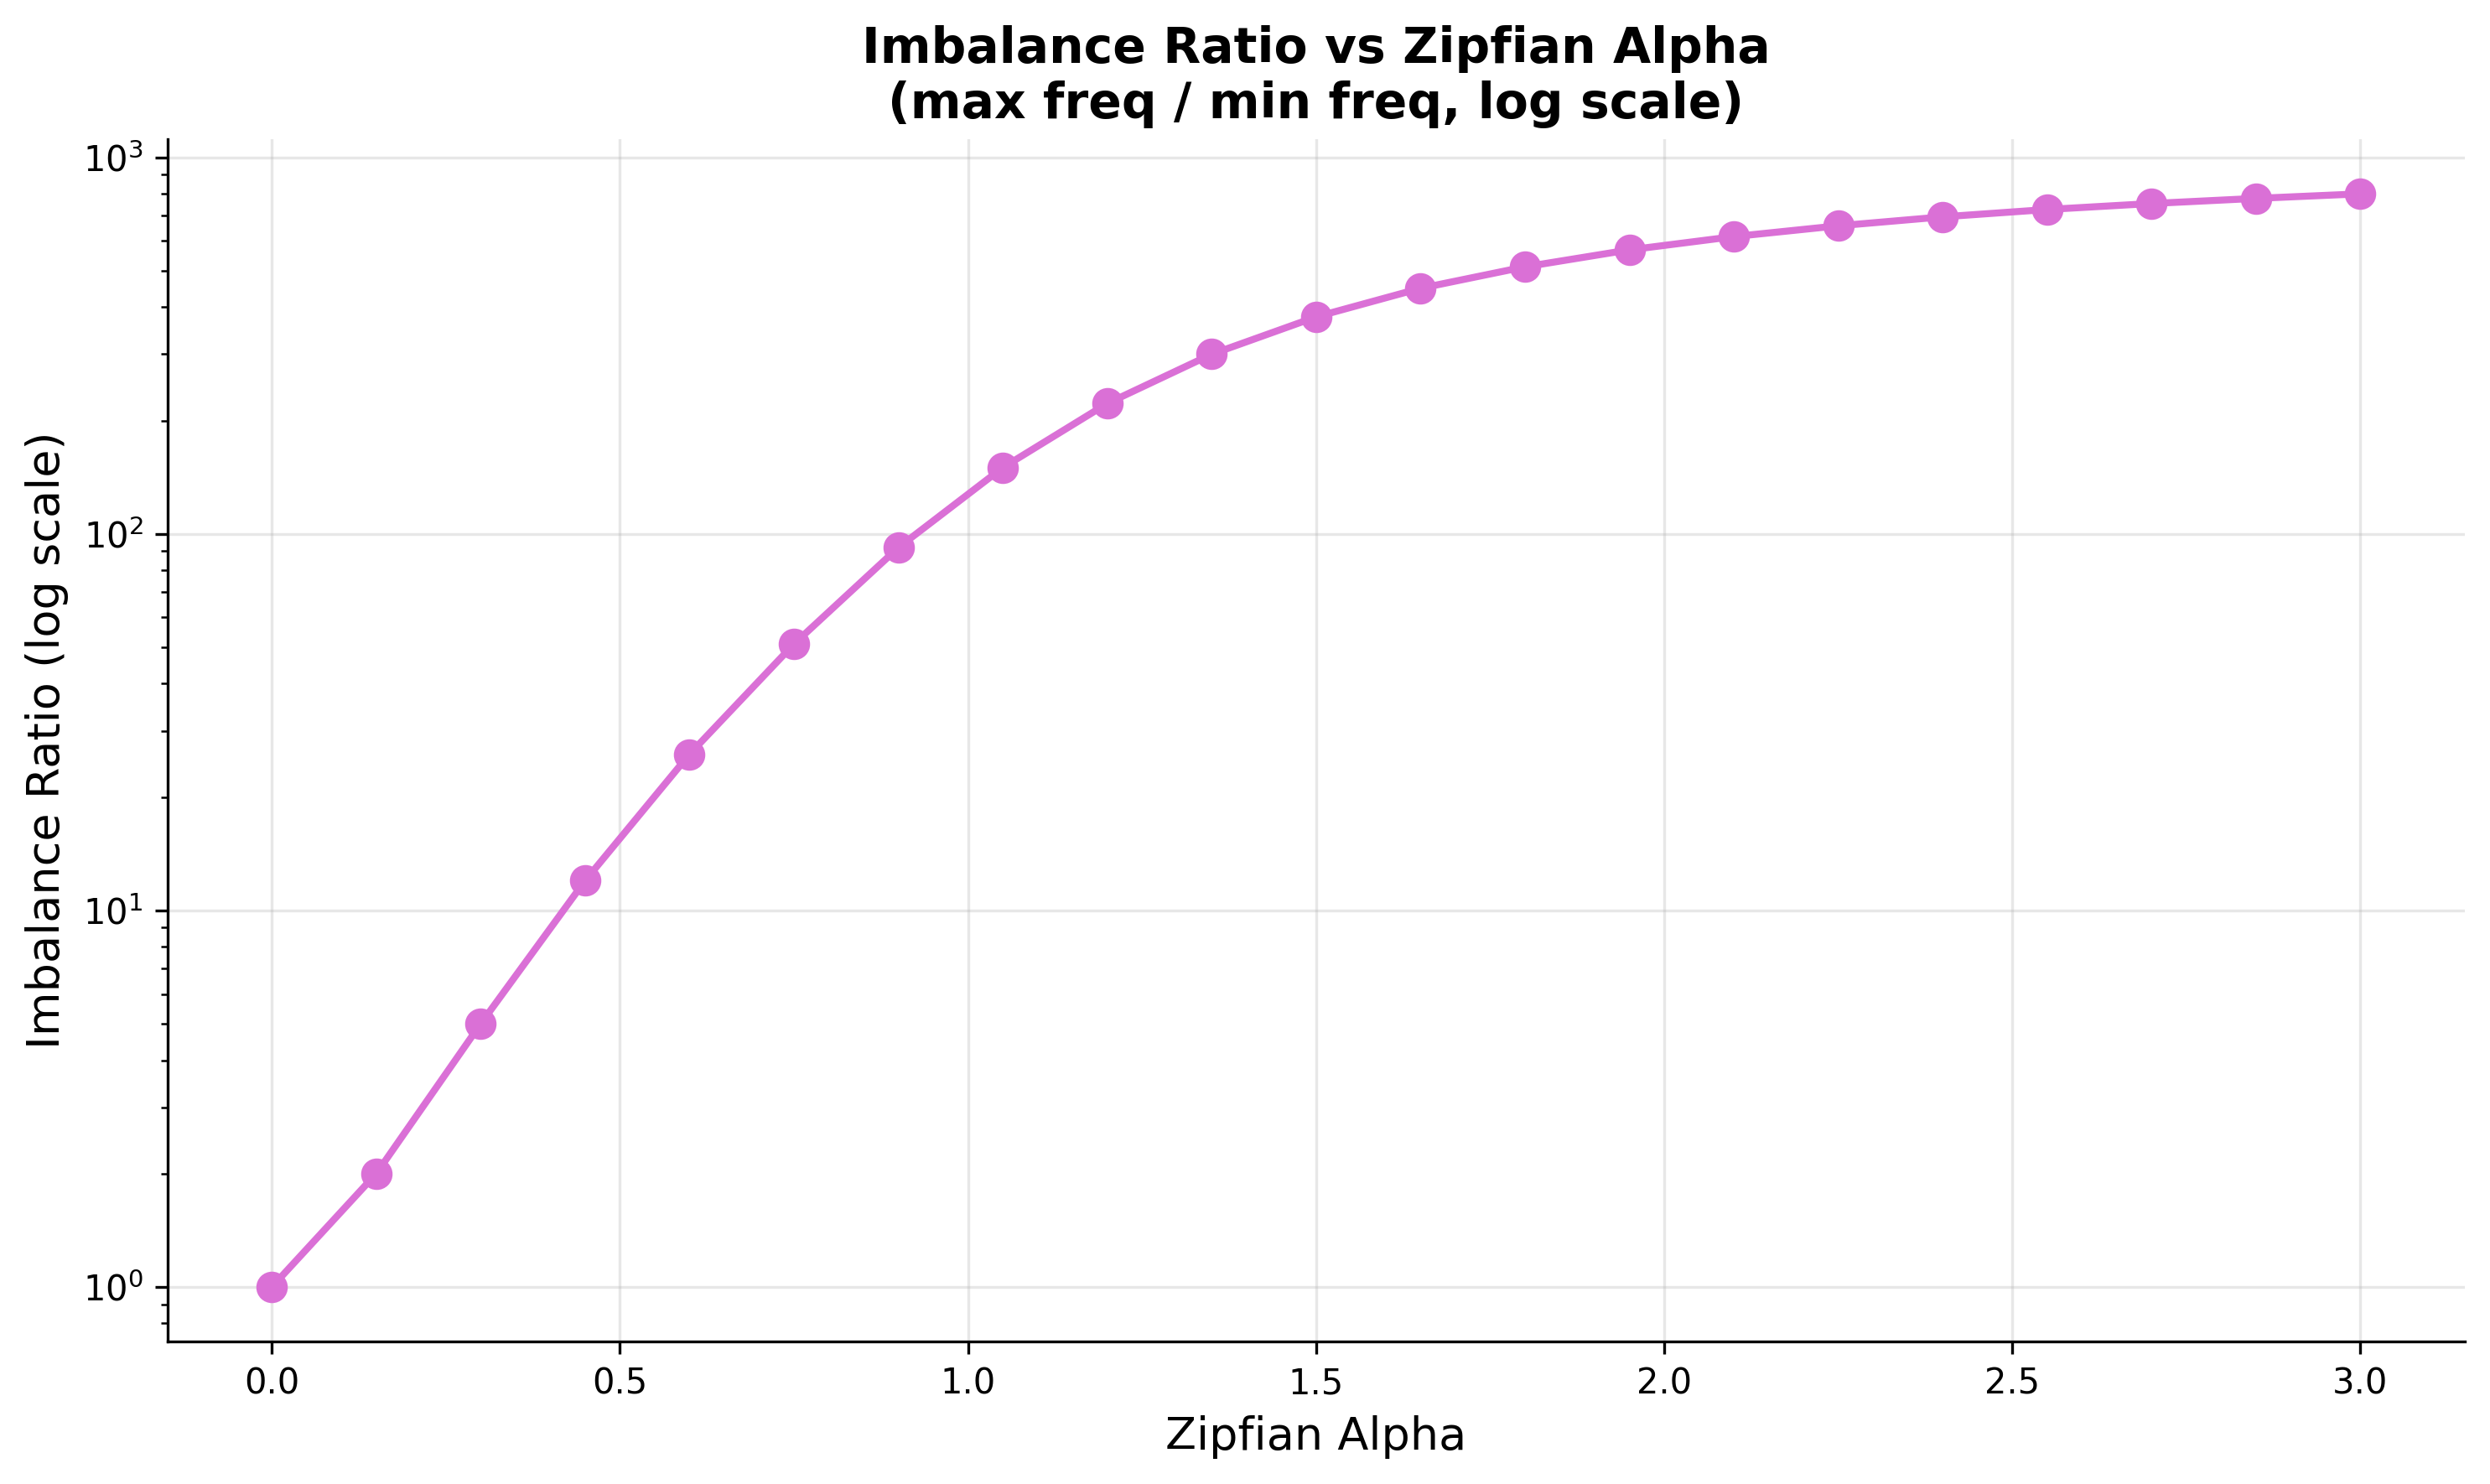
\includegraphics[width=0.95\textwidth]{images/appendix_imbalance_ratio_vs_alpha.png}%
    }{%
        \fcolorbox{red}{white}{\parbox[c][0.14\textheight][c]{0.9\textwidth}{\centering\textcolor{red}{Placeholder figure\\\texttt{\detokenize{images/appendix_imbalance_ratio_vs_alpha.png}}}}}%
    }
    \caption{Imbalance ratio of the pair frequency distribution as a function of $\alpha$, computed on the training set of seed 42.}
    \label{fig:appendix-imbalance-ratio-vs-alpha}
\end{figure}

The imbalance ratio grows sharply with $\alpha$. At low concentration the most frequent pair appears roughly three times as often as the rarest; at high concentration the gap grows beyond an order of magnitude. Of the four measures this is the one that responds most sharply to the tail, which is precisely where the Zipfian construction does most of its work.

\section{Consistency of the Four Metrics}
\label{sec:appendix-metric-consistency}

The four metrics all move in the direction consistent with a single interpretation: as $\alpha$ grows, a smaller subset of pairs accounts for a larger share of the total training exposures. They differ in what they emphasise, total uncertainty for Shannon, effective diversity for Simpson, aggregate inequality for Gini, and tail asymmetry for the imbalance ratio, but their qualitative agreement across the $\alpha$ range confirms that the Zipfian construction produces the intended monotone concentration effect.

\section{Per-$\alpha$ Snapshots of the KL Divergence}
\label{sec:appendix-kl-snapshots}

The KL divergence discussion in Chapter~\ref{ch:technical} uses a single aggregate summary. This section reports the per-$\alpha$ snapshots of the underlying MDL score distributions for a representative seed, showing how the subsequence distribution reshapes progressively as concentration $\alpha$ grows.

Each snapshot compares the MDL distribution at that $\alpha$ against the uniform baseline ($\alpha = 0.00$), sorted independently for each curve by the subsequence's own rank in that distribution. The log-scale plot makes the shape of each distribution clear: uniform distributions are broad and heavy-tailed, while concentrated distributions have a much steeper drop-off after the first few dominant subsequences. The KL divergence value reported in each title quantifies the total departure from the uniform baseline.

\begin{figure}[htbp]
    \centering
    \IfFileExists{images/appendix_kl_alpha_060.png}{%
        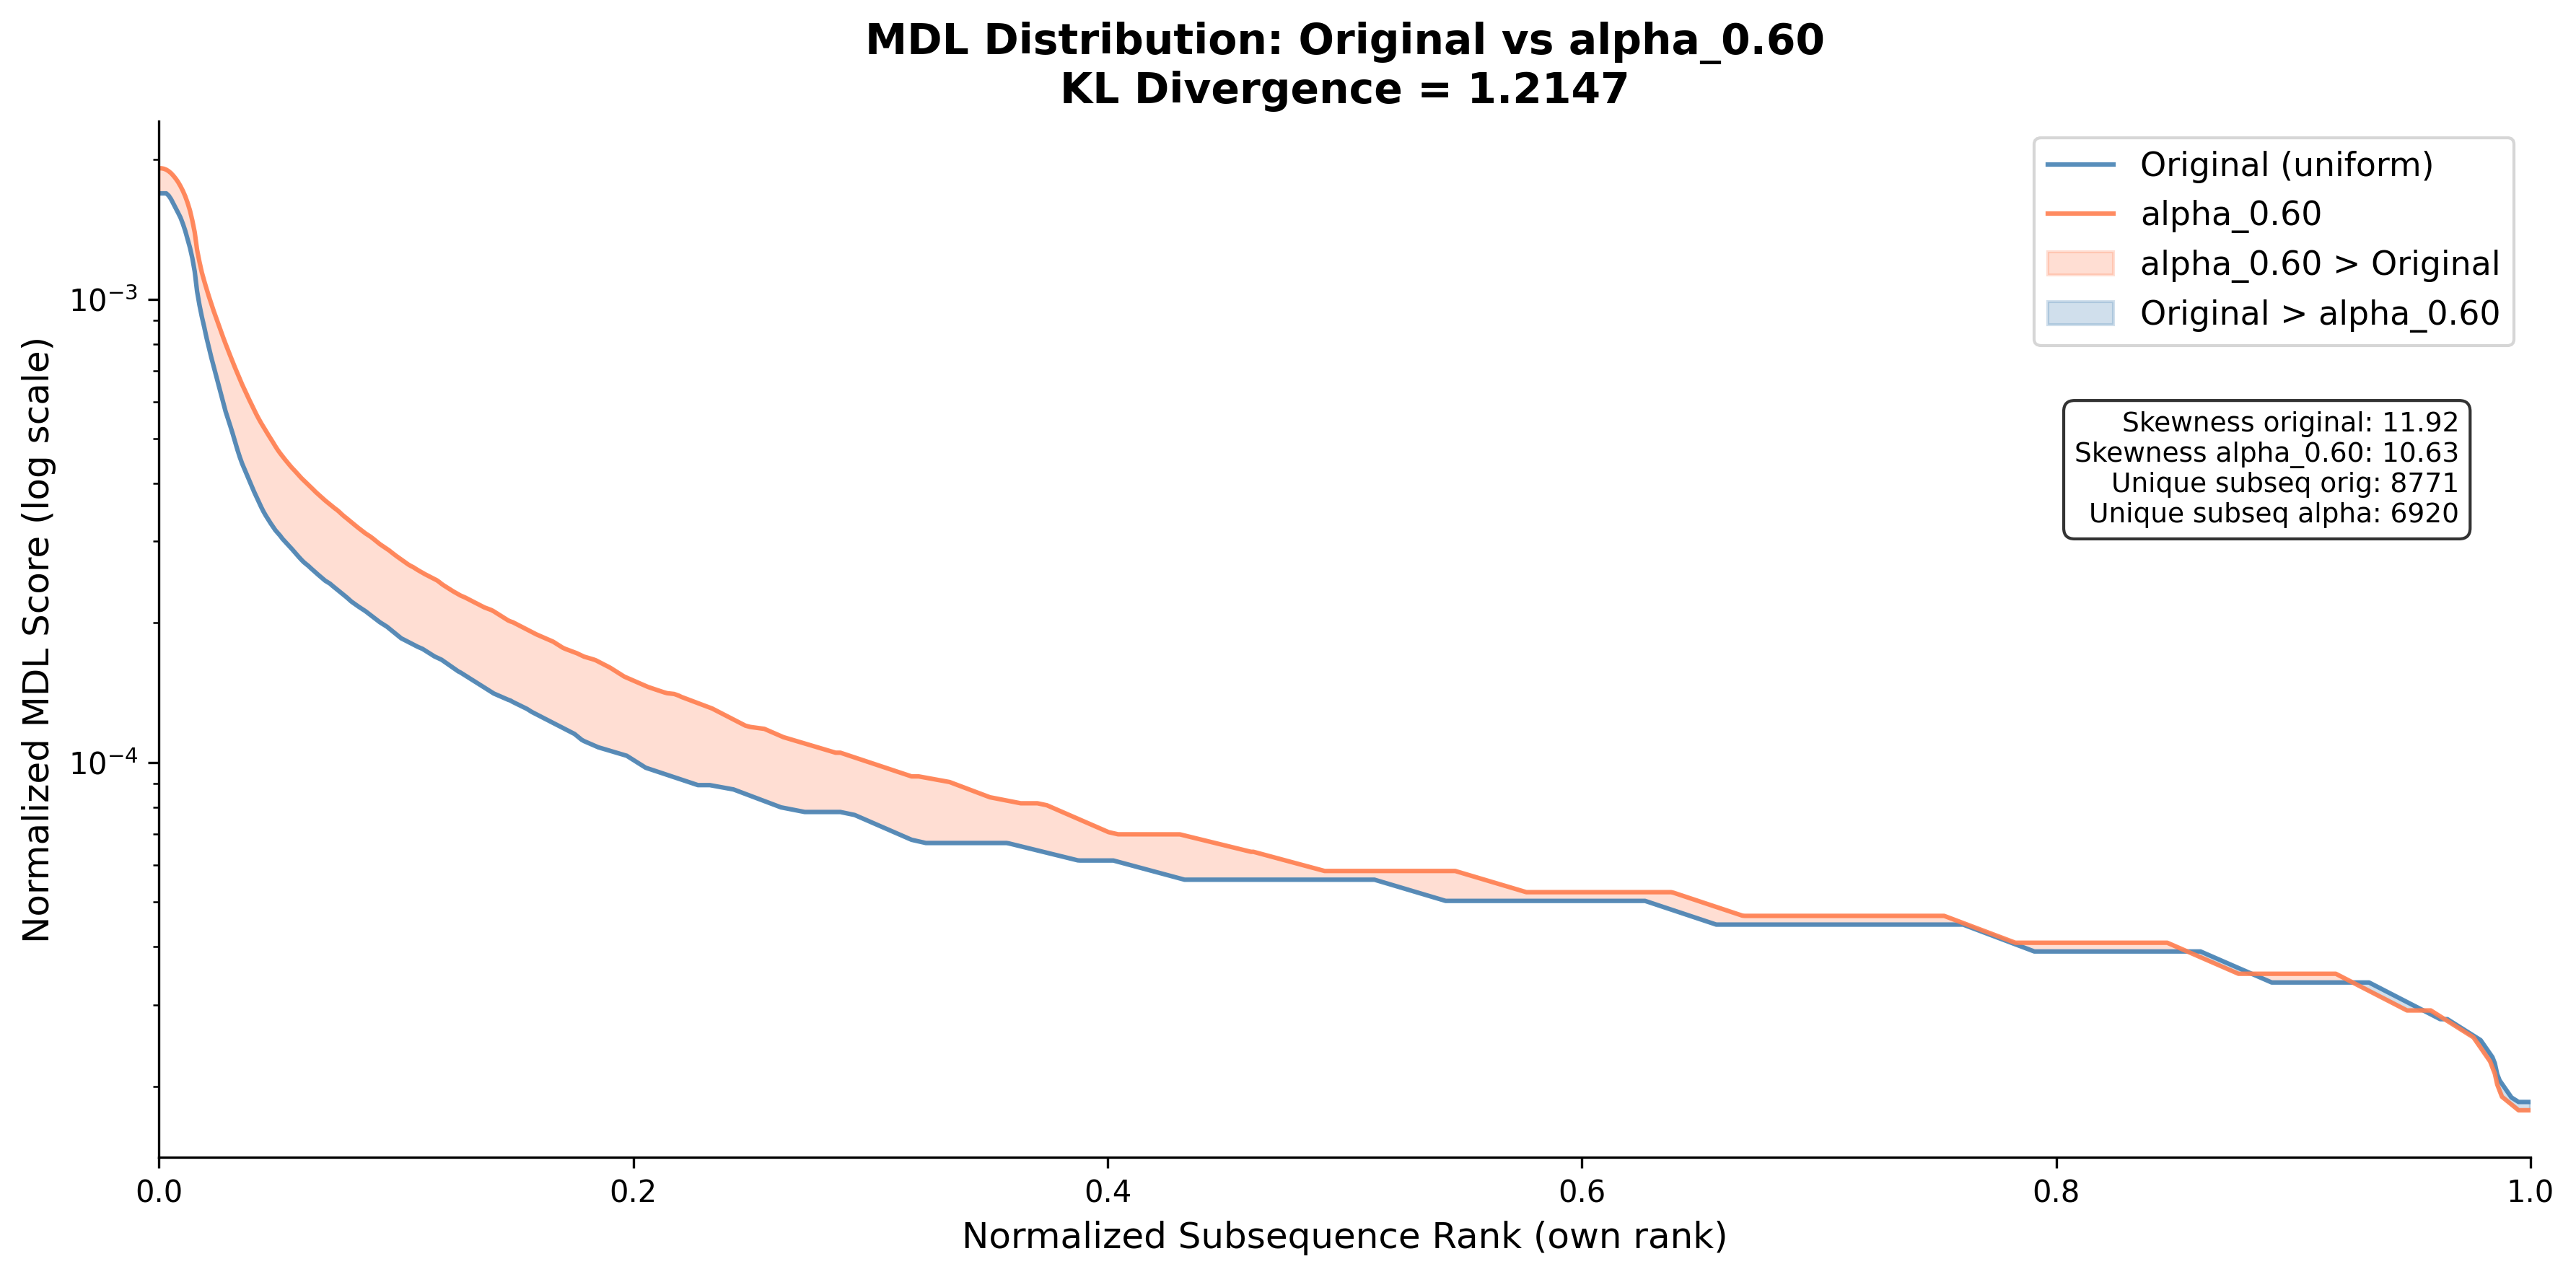
\includegraphics[width=0.95\textwidth]{images/appendix_kl_alpha_060.png}%
    }{%
        \fcolorbox{red}{white}{\parbox[c][0.14\textheight][c]{0.9\textwidth}{\centering\textcolor{red}{Placeholder figure\\\texttt{\detokenize{images/appendix_kl_alpha_060.png}}}}}%
    }
    \caption{MDL distribution at $\alpha = 0.60$ compared to $\alpha = 0.00$ (uniform).}
    \label{fig:appendix-kl-alpha-060}
\end{figure}

\begin{figure}[htbp]
    \centering
    \IfFileExists{images/appendix_kl_alpha_180.png}{%
        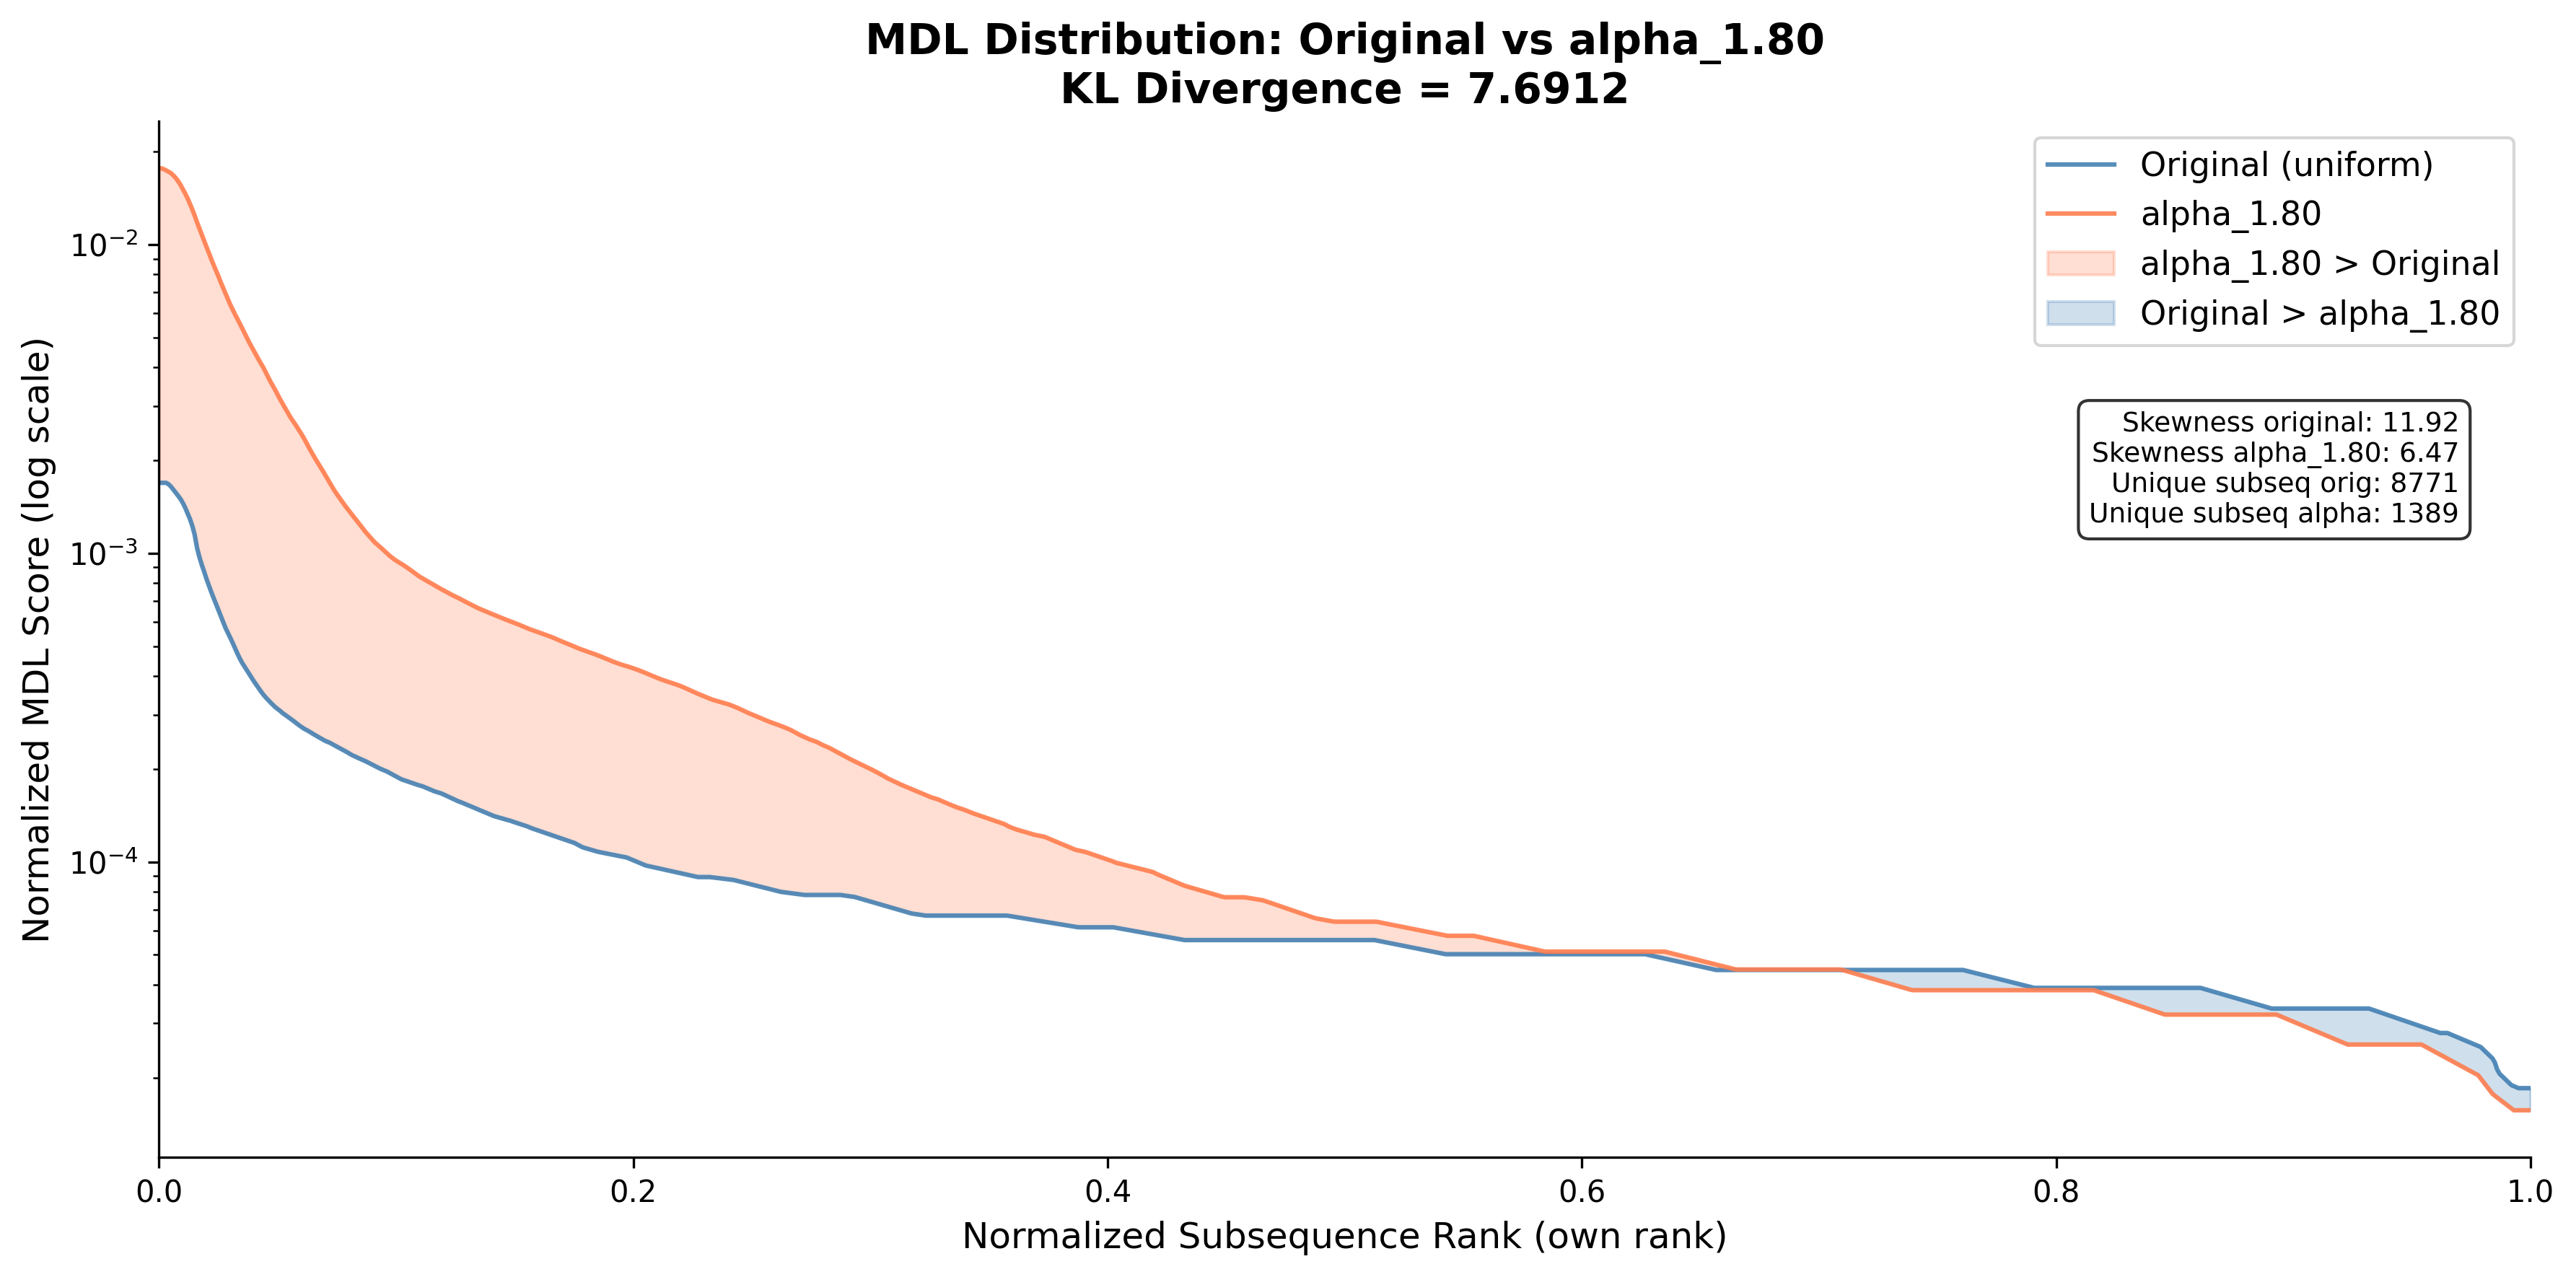
\includegraphics[width=0.95\textwidth]{images/appendix_kl_alpha_180.png}%
    }{%
        \fcolorbox{red}{white}{\parbox[c][0.14\textheight][c]{0.9\textwidth}{\centering\textcolor{red}{Placeholder figure\\\texttt{\detokenize{images/appendix_kl_alpha_180.png}}}}}%
    }
    \caption{MDL distribution at $\alpha = 1.80$ compared to $\alpha = 0.00$ (uniform).}
    \label{fig:appendix-kl-alpha-180}
\end{figure}

\begin{figure}[htbp]
    \centering
    \IfFileExists{images/appendix_kl_alpha_300.png}{%
        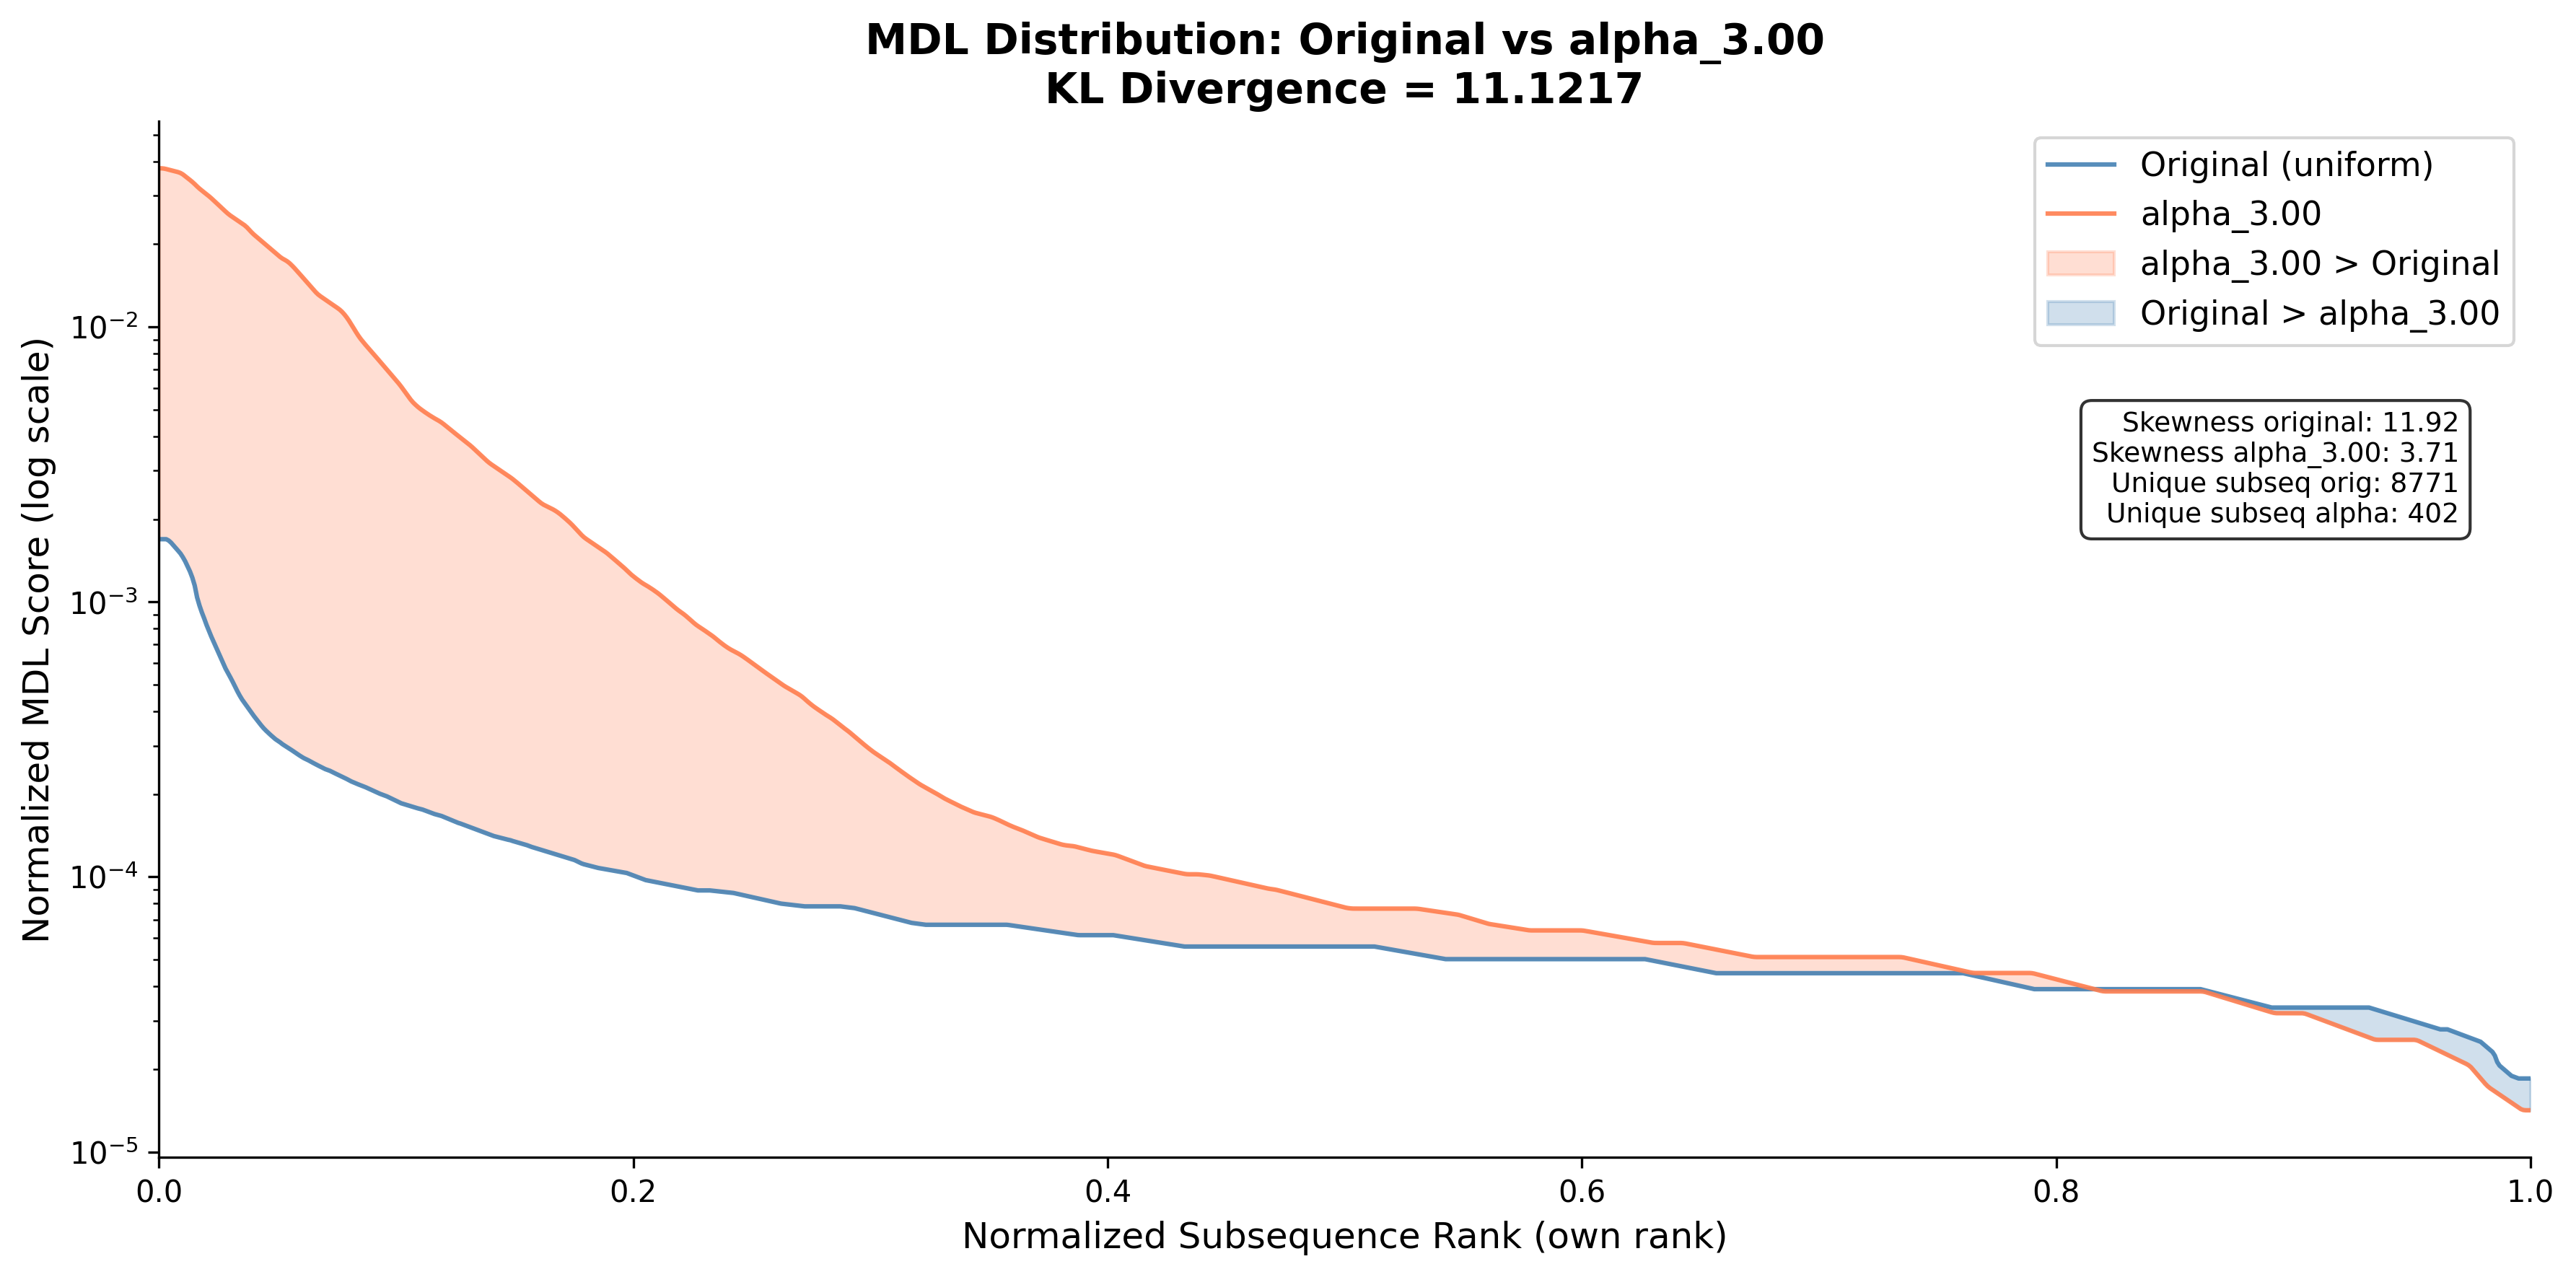
\includegraphics[width=0.95\textwidth]{images/appendix_kl_alpha_300.png}%
    }{%
        \fcolorbox{red}{white}{\parbox[c][0.14\textheight][c]{0.9\textwidth}{\centering\textcolor{red}{Placeholder figure\\\texttt{\detokenize{images/appendix_kl_alpha_300.png}}}}}%
    }
    \caption{MDL distribution at $\alpha = 3.00$ compared to $\alpha = 0.00$ (uniform).}
    \label{fig:appendix-kl-alpha-300}
\end{figure}

The three snapshots trace out a coherent progression. At $\alpha = 0.60$, the two curves are close throughout most of their range and the KL is modest. At $\alpha = 1.80$, the concentrated distribution dominates the uniform one across the entire body of the ranking, and the KL is substantial. At $\alpha = 3.00$, the two distributions become almost disjoint: the concentrated one has very few unique subsequences (a fraction of the roughly 8771 that appear under the uniform baseline), and those that survive have MDL scores an order of magnitude higher than under the uniform baseline.
\section{Alternative Visualisations of the KL Divergence}
\label{sec:appendix-kl-alternative-visualisations}

The KL snapshots reported in Section~\ref{sec:appendix-kl-snapshots} use a log-scale representation with each distribution sorted independently by its own rank. For completeness, we include two alternative visualisations of the same underlying data. The linear-scale version aligns both curves on the union of all observed subsequences, making the redistribution of probability mass explicit. The CDF version tracks how much of the total MDL mass is captured by the top-$k$ subsequences, so concentration appears as a steep early rise followed by a quick plateau.

\begin{figure}[htbp]
    \centering
    \IfFileExists{images/appendix_kl_linear_alpha_180.png}{%
        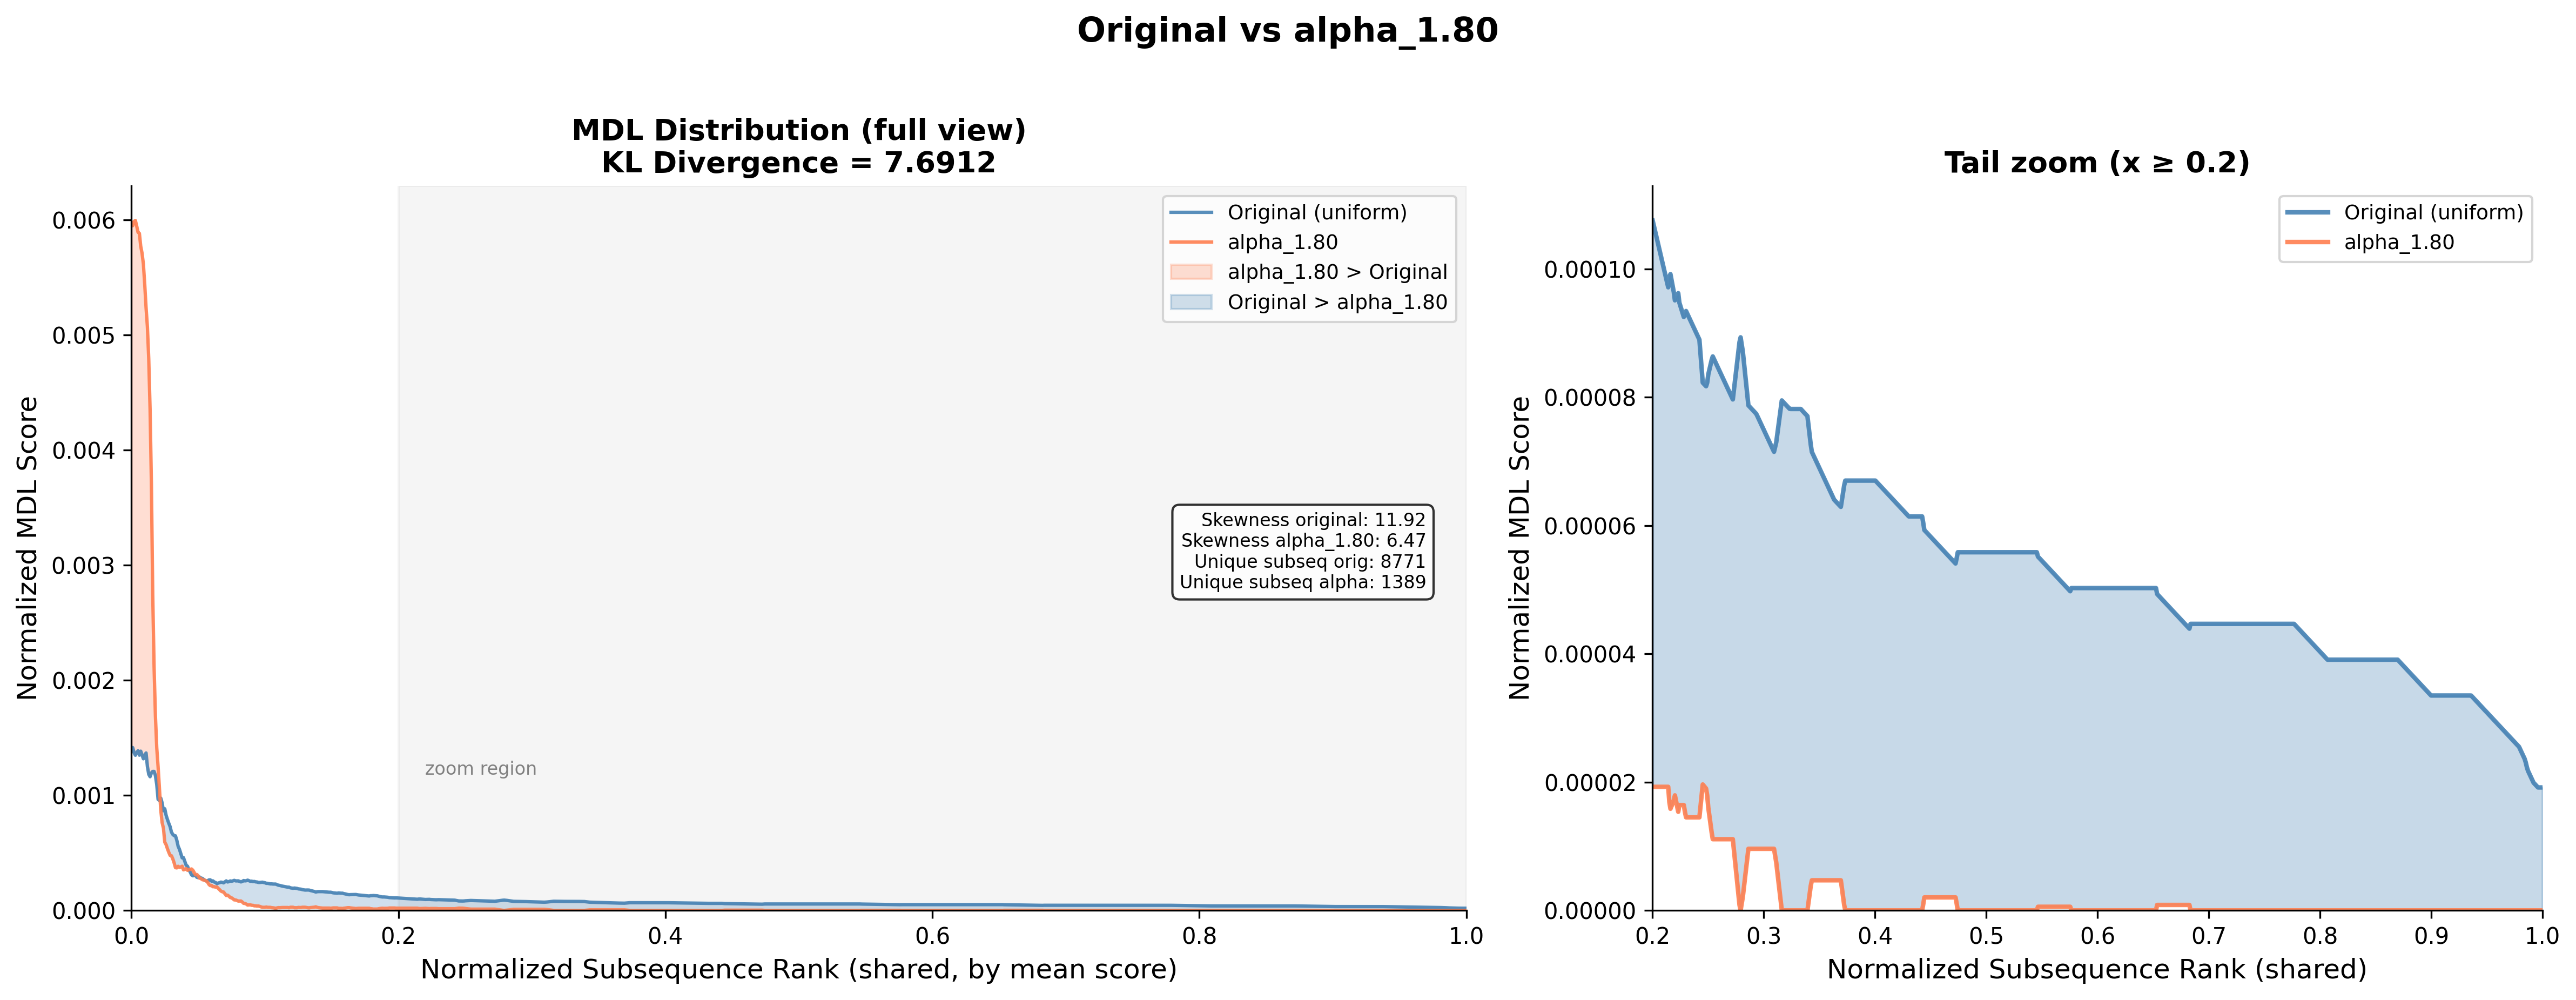
\includegraphics[width=0.95\textwidth]{images/appendix_kl_linear_alpha_180.png}%
    }{%
        \fcolorbox{red}{white}{\parbox[c][0.14\textheight][c]{0.9\textwidth}{\centering\textcolor{red}{Placeholder figure\\\texttt{\detokenize{images/appendix_kl_linear_alpha_180.png}}}}}%
    }
    \caption{Linear-scale KL comparison at $\alpha = 1.80$ (seed 42), with both curves aligned on the union of all observed subsequences.}
    \label{fig:appendix-kl-linear-alpha-180}
\end{figure}

\begin{figure}[htbp]
    \centering
    \IfFileExists{images/appendix_kl_cdf_alpha_180.png}{%
        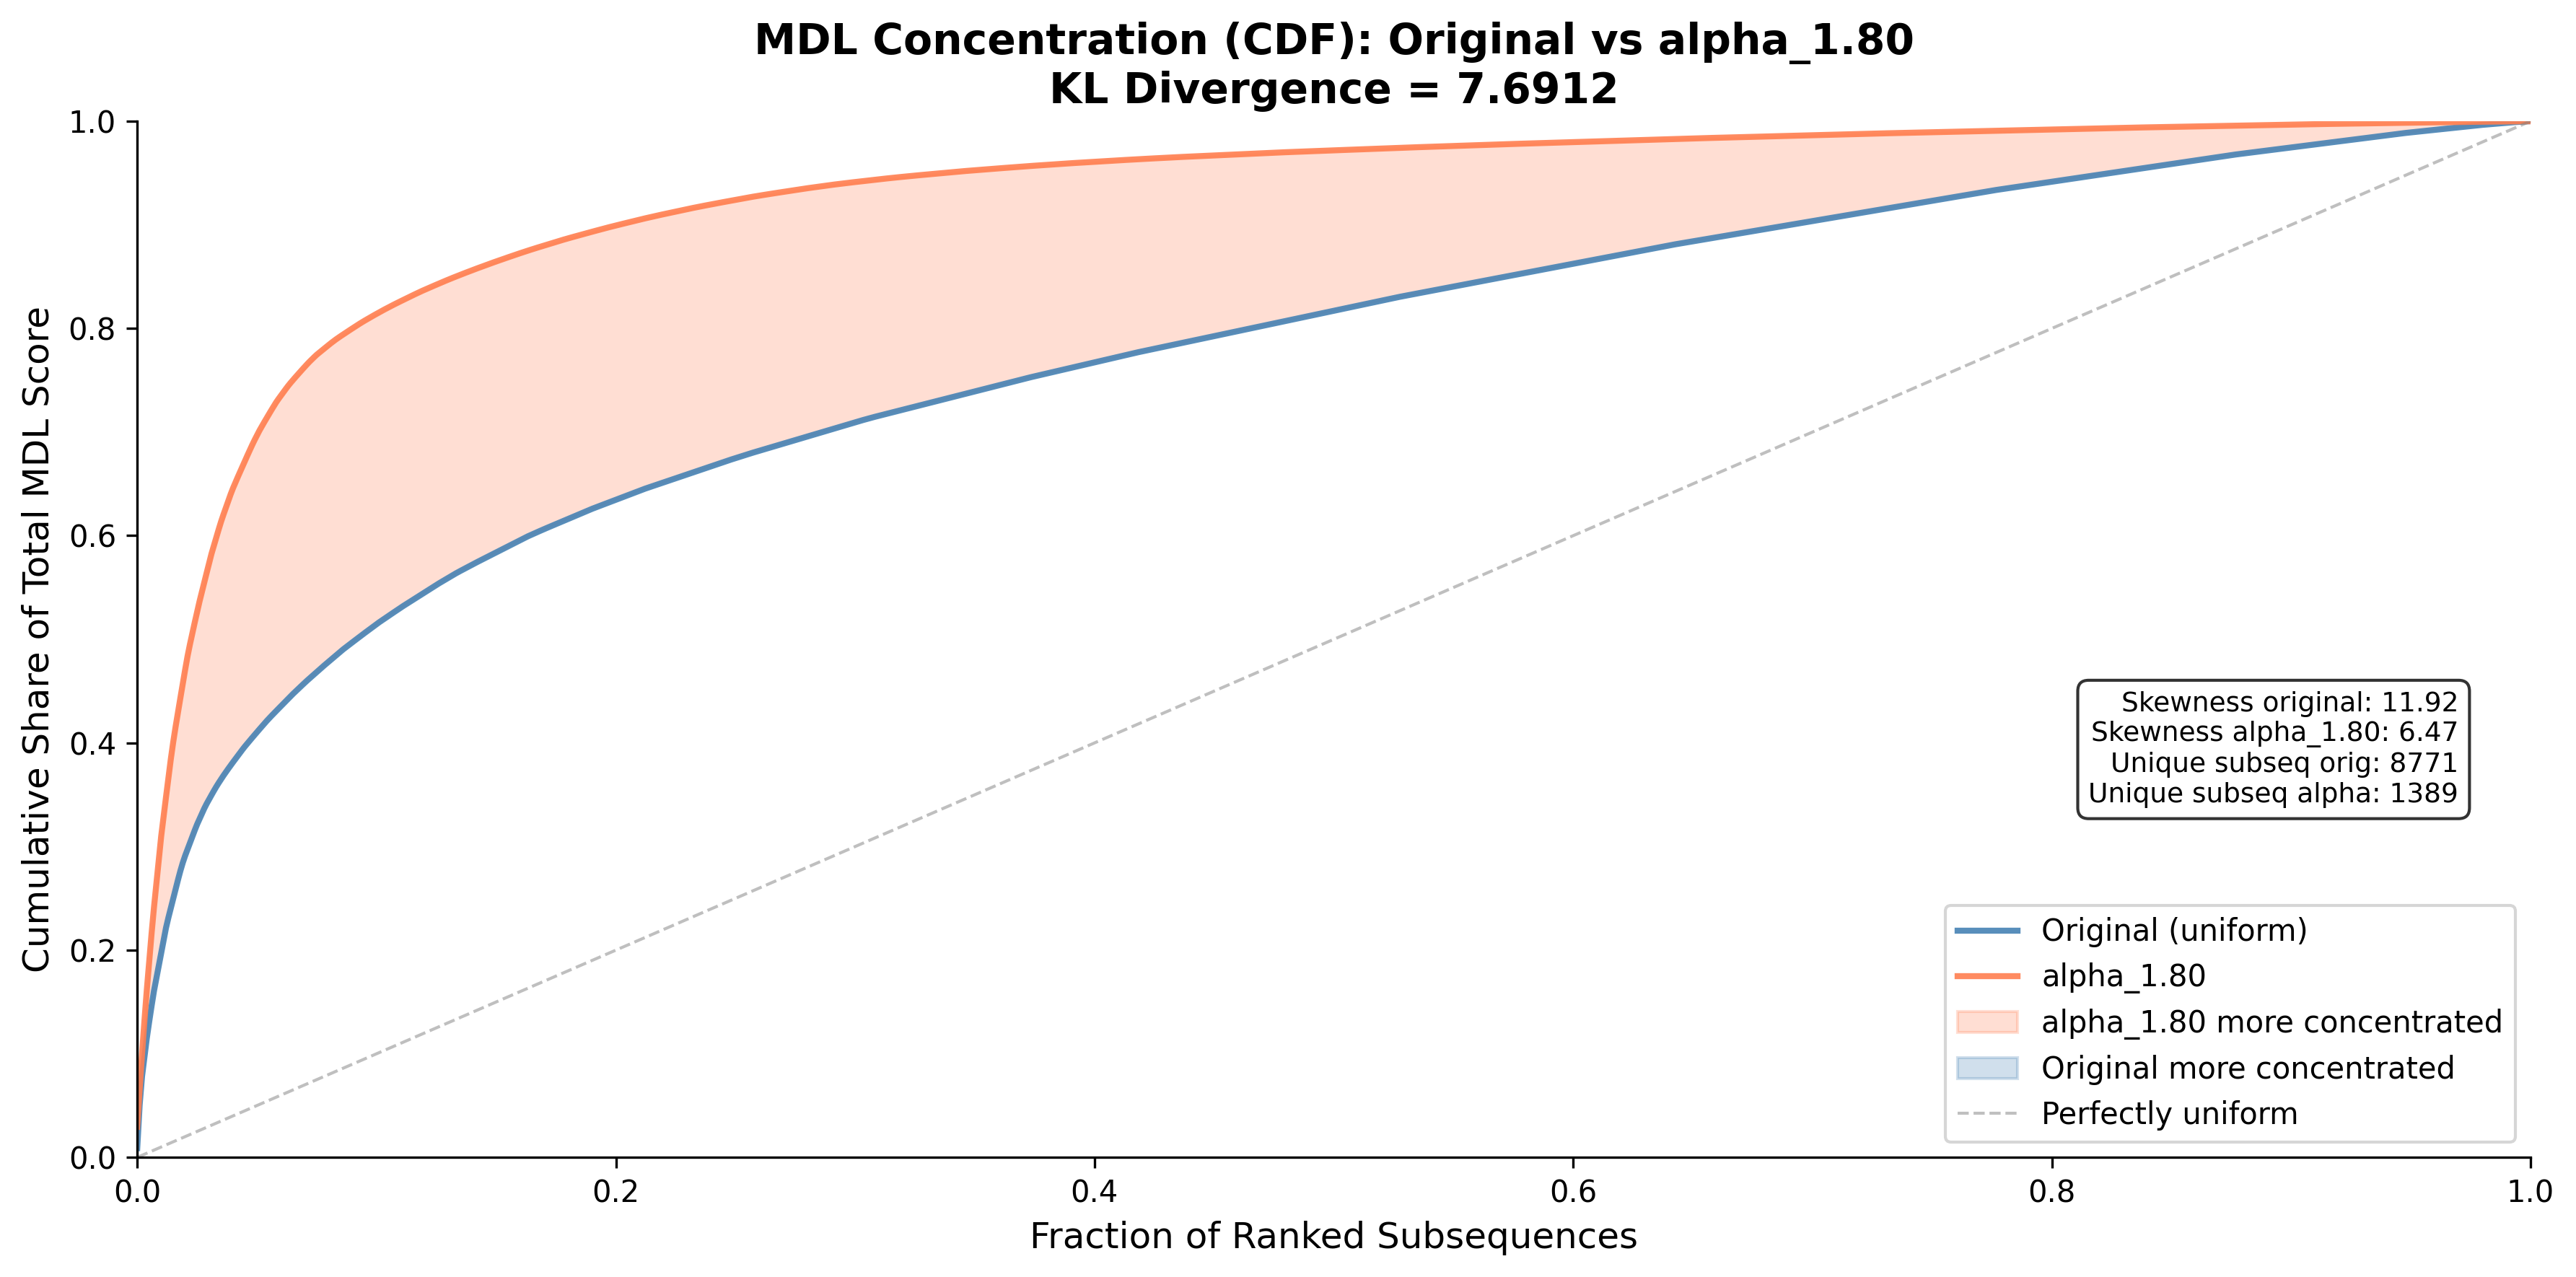
\includegraphics[width=0.95\textwidth]{images/appendix_kl_cdf_alpha_180.png}%
    }{%
        \fcolorbox{red}{white}{\parbox[c][0.14\textheight][c]{0.9\textwidth}{\centering\textcolor{red}{Placeholder figure\\\texttt{\detokenize{images/appendix_kl_cdf_alpha_180.png}}}}}%
    }
    \caption{CDF-based KL comparison at $\alpha = 1.80$ (seed 42).}
    \label{fig:appendix-kl-cdf-alpha-180}
\end{figure}

Both alternatives lead to the same qualitative conclusion as the main representation: as $\alpha$ grows, the concentrated distribution places substantially more mass on the top-ranked subsequences and substantially less on the rest, with a KL divergence that grows steadily throughout the $\alpha$ range.